\documentclass[a4paper,10pt,twocolumn,uplatex]{jsarticle}
\usepackage{style/nislab,style/resume}

%---------------------------------------------------------------------
% レジュメ種別・日付設定(要変更)
% \type{} 1:修士論文諮問会 2:卒業論文発表会 3:月例発表会 4:研究室合同発表会
%---------------------------------------------------------------------
\type{3}
\year{2022}
\month{6}
\date{11}

%---------------------------------------------------------------------
% ページ番号設定(要変更)
%---------------------------------------------------------------------
\setcounter{page}{1}

%---------------------------------------------------------------------
% 変更不要
%---------------------------------------------------------------------
\begin{document}

%---------------------------------------------------------------------
% タイトル作成部分(要変更)
% \maketitle{タイトル}{title}{名前}{name}
%---------------------------------------------------------------------
\maketitle{タイトルタイトルタイトルタイトルタイトルタイトル}
{Title Title Title Title Title Title}
{竹内 一真}
{Kazuma Takeuchi}

% --------------------------- Section1  ---------------------------

\section{はじめに}
近年,多方面でのドローンを活用した事業が進出しており,インフラ点検や災害調査など,応用分野を拡大しながら,世界のドローン市場は急速に成長している\cite{Nonami}.
中でも小型ドローンの特徴である機体の大きさを活かして,人間が入れないような狭い空間での活躍の場も増加している.
しかし,狭小空間でのドローン飛行は,遮蔽物が多く,操縦者は遮られた視点からの操縦を必要とする.
そのため,死角領域内のドローン操縦では,ドローンを視認できない中,衝突することなく,安全に操縦する技術が求められる.
\par
オンボードカメラ搭載ドローンを使用する場合では,操縦者は,ドローンから送られる空撮した映像を元に操縦が可能となる.
このようなドローン操縦方法では,実際の現実空間を映像として見ながら操縦できるため,現実のドローンを視認することなく,狭小空間を探索することができる.
しかし,カメラが前方しか写さないことにより,前方以外の死角が多くなり,状況認識が不十分となるため\cite{Green},狭小空間のように狭く,障害物が多いような環境では,操縦は困難である.
大型ドローンでは,自律飛行や障害物回避などの機能が実現されているが,センサ搭載制限のある小型ドローンでは,障害物回避の支援がないことが多く,衝突の危険性があり,
また,障害物回避の機能を搭載していても,狭小空間では障害物回避が行えない場面が多く存在する\cite{syohou}.
\par
そこで,Augmented Reality(AR)を用いて死角領域内を可視化することで,ドローンの操縦性向上や安全性向上が期待されている\cite{Erat}.
事前に走行環境をマッピングすることで3次元環境地図を取得し,空間認識を提供している.
しかし,狭小空間のドローン操縦において,事前に3次元環境地図を用意することは困難なため,
走行環境を探索する中で,リアルタイムにマッピングを行う必要がある.また,複数ドローンが混在する場合も問題である.
各ドローンがマッピングした3次元環境地図が異なるため,精度が悪く,操縦者の空間認識に悪影響を及ぼすため,作成した3次元環境地図を
統一し,精度を向上する必要がある.
% 操縦者視点でドローンを視認し飛行させる三人称視点操縦の場合では,ドローン中心の一人称視点での操縦に比べて,ドローン周辺の状況を把握することができ,また,ドローンの実際の高さや位置を正確に把握することができる\cite{Green}.
% しかし,三人称視点操縦では,操縦者から見えるドローンまでの距離感が掴めないため\cite{Zollmann},ドローン周辺の障害物へ衝突する恐れがある.
% 大型ドローンでは,自律飛行や障害物回避などの機能が実現されているが,センサ搭載制限のある小型ドローンでは,障害物回避の支援がないことが多く,衝突の危険性がある.
% また,障害物回避を搭載していても,狭小空間では障害物回避が行えない場面が多く存在する\cite{syohou}.
本研究では,狭小空間による死角領域内の複数ドローン飛行の危険性を軽減するため,ARにより操縦者の死角領域内を可視化し,リアルタイムに3次元環境地図を作成し,合成するシステムを開発する.

% --------------------------- Figure  ---------------------------

\begin{figure}[!tb]
  \centering
  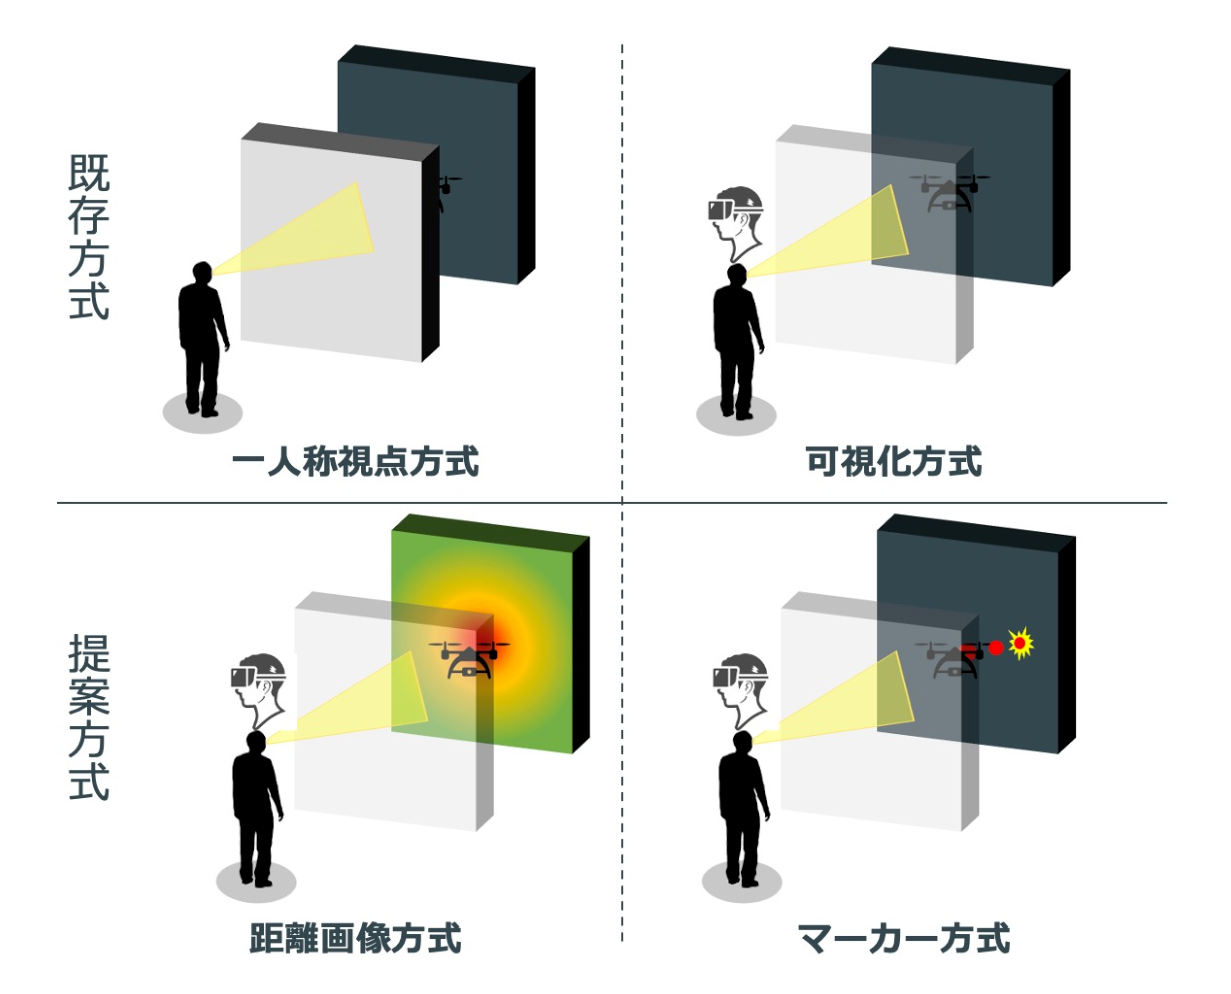
\includegraphics[width=\linewidth]{img/03_outline.eps}
  \caption{悩む男の子}
  \label{fig:sample1}
\end{figure}

% \begin{figure*}[!tb]
%   \centering
%   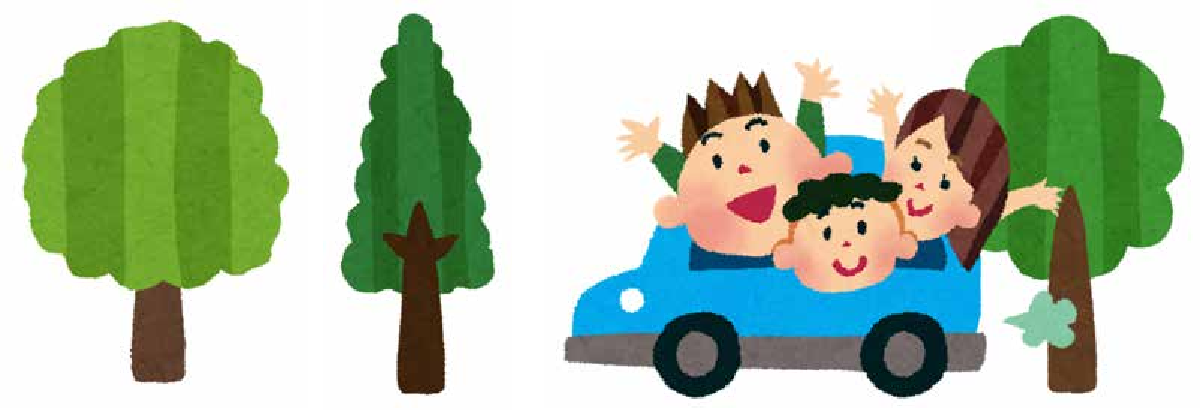
\includegraphics[width=\linewidth]{img/sample2.pdf}
%   \caption{ドライブする家族}
%   \label{fig:sample2}
% \end{figure*}

% --------------------------- Section2  ---------------------------

\section{提案システム}
\subsection{概要}
本研究では,狭小空間により,操縦者と小型ドローン(以下,ドローン)の間に遮蔽物があり,ドローンを視認できない環境を「死角領域」とする.
図\ref{fig:03_enviroment}の環境におけるドローン操縦を想定しており,各ドローンがリアルタイムで飛行環境をマッピングし作成された3次元環境地図
を,ARにより重畳表示することで,死角領域内の空間認識を提供している.
\par

\subsection{死角領域内のAR可視化}
先に述べた先行研究\cite{Erat}を元に,操縦者に死角領域内の空間認識を提供する.
ドローンと操縦者の間に遮蔽物が存在すると判断した際,ドローンが飛行している場所を操縦者にとっての死角領域とし,
マッピングした三次元環境地図における遮蔽物を透過した上で,現実環境に重畳表示することで,仮想的に死角領域を可視化している.
操縦者は,死角領域内を飛行するドローンを視認することはできないが,ARによって仮想のドローンと,ドローン周辺の三次元環境を視認することができる.

\subsection{3次元環境地図の生成}
本研究におけるドローン操縦では,リアルタイムでマッピングを行い,3次元環境地図を作成する必要がある.
本来の3次元地図はセンサーデータの重ね合わせによって生成しており,膨大な数の点の集合であり,
データ量が非常に大きいため,ARに与える負荷が大きい.
そのため,3DマッピングフレームワークであるOctoMapを用いることで,簡易的に3次元環境地図を生成する.
各ドローンはVisual SLAMであるORB-SLAM2を用いて,カメラで取得した画像から特徴点自己位置推定を行い,
周囲の環境の3Dポイントクラウドを取得する.
取得した3DポイントクラウドをOctoMapを用いて3次元環境地図を生成することで,ドローン周辺の環境を仮想的に提供する.
また,各ドローンの位置情報,生成した各3次元環境地図は個々で独立している.そこで,各ドローンをワールド座標系で管理する.
その上で,3次元環境地図が重なる場合には,3Dポイントクラウドを合成しOctoMapに変換することで,より精度を高めた共通の3次元環境地図を生成する.
% --------------------------- Section3  ---------------------------

\section{評価}

\subsection{実装環境}
システム構成を図\ref{fig:04_system}に示す.
使用するドローンはRyze Tech社製Tello EDU(以下,Tello)を用いる.Telloはプログラミングによってフライトコントロールを行うことができ,
規定のコマンドを送信することで飛行制御することができる.
\par
ARHMDはMicrosoft HoloLens2(以下,HoloLens)を使用する.
システムはHoloLens2上でUnityアプリケーションが動作しており,Unity内で仮想ドローン,3次元環境地図を配置する.
\par
サーバではTello,HoloLensとUDP通信を行なっており,常時,Telloの位置情報をHoloLensに送信する.
Telloより受け取った値をUnity座標系へ変換し,変換後の値を反映させることにより,仮想ドローンの位置合わせを行なっている.
% ここでUDPを使用する理由として,Tello,サーバ,HoloLens間の遅延低減を目的とする.
\par


% --------------------------- Figure  ---------------------------

\begin{figure}[!tb]
  \centering
  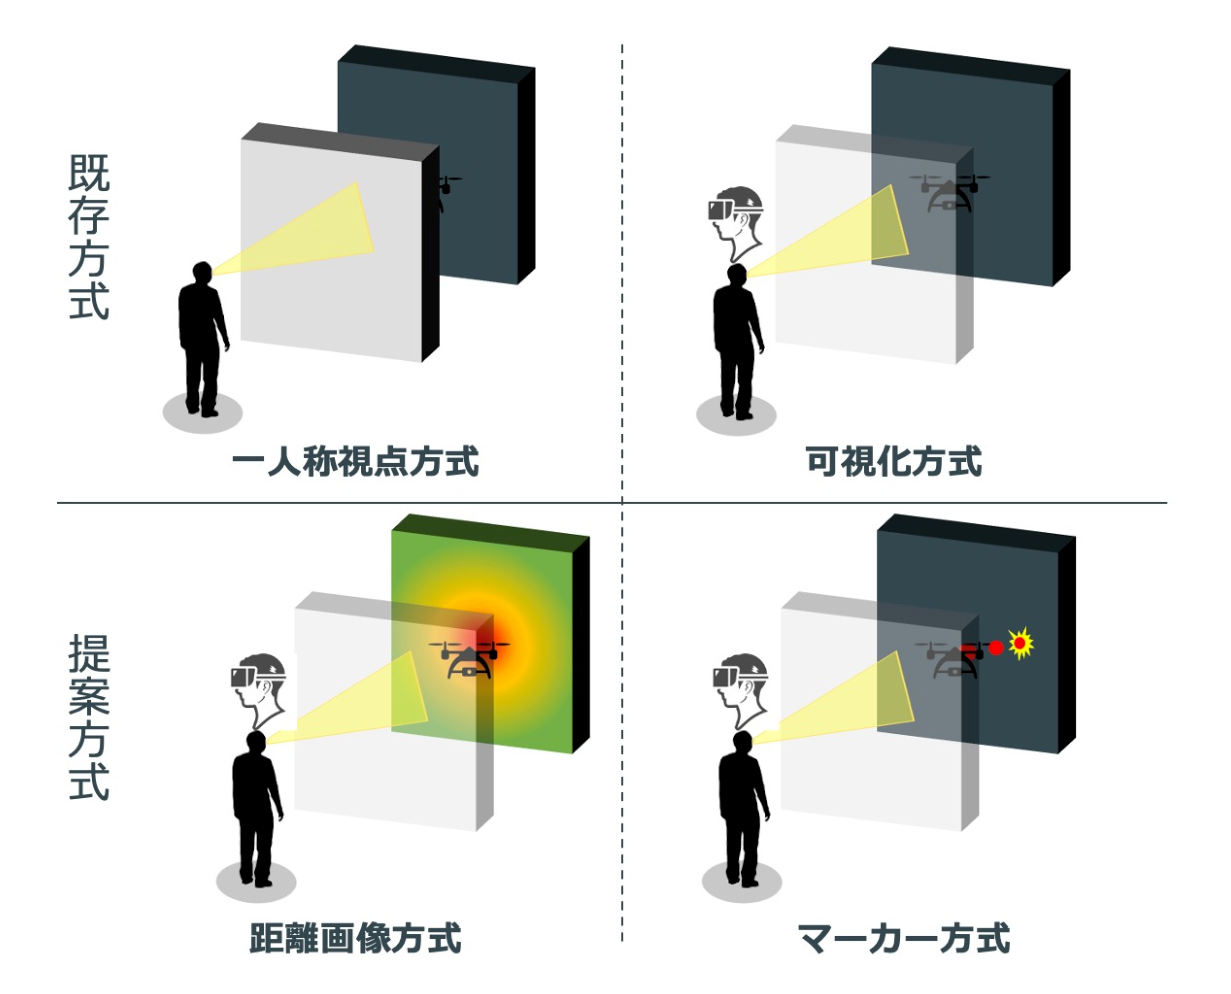
\includegraphics[width=\linewidth]{img/03_outline.eps}
  \caption{悩む男の子}
  \label{fig:sample1}
\end{figure}
  
% -----------------------------------------------------------------

\subsection{実験}
死角領域内を飛行するドローンの操縦において,各方式がどのような影響を与えるかを評価するため,実験協力者による実験を行う.
実験参加者はドローンをスタート地点から目的地まで操縦し,目的地点で着陸するタスクを行う.
実験では従来のFPVによるドローン視点をもとに飛行する操縦手法,死角領域内を可視化した操縦手法,複数ドローンの3次元環境地図を合成した操縦手法の計3つの手法で実験を行う.



\subsection{評価項目}
本提案手法を用いることによって狭小空間探査を手軽に安全に行え
るかを検証するため,主観的評価と客観的評価を行う.主観的評価として参加者へのアンケート,
客観的評価として操縦者がタスクを完了するまでの平均操縦時間,障害物への平均衝突回数,ドローン移動コマンドの平均間隔時間を評価する.
% -----------------------------------------------------------------

% --------------------------- Section4  ---------------------------

\section{おわりに}

小型ドローンは機体の大きさを活かして,インフラ点検や災害調査のような,人間が立ち入れない狭小空間での活躍が増えている.
しかし,狭小空間でのドローン飛行では,遮蔽物による視点が遮られる死角領域内での操縦を必要とする.
また,従来の操縦法では状況認識が不十分であるため,ドローン周辺に位置する障害物が多い狭小空間では,ドローン操縦は困難である.\par
遮蔽物,障害物が多い狭小空間では,死角領域内におけるドローン飛行の危険性を軽減する必要がある.
そこで本研究では,各ドローンがリアルタイムで飛行環境をマッピングし作成された3次元環境地図をもとに,ARにより操縦者の死角領域内に存在するドローンと周辺環境を可視化するARシステムを提案する.
本提案システムについて,死角領域内でのドローン操縦性を評価実験する.

%---------------------------------------------------------------------
% Bibliography(参考文献)
%---------------------------------------------------------------------
% thebibliography を利用する場合は以下を使用
\footnotesize{
  \begin{thebibliography}{99}
    \bibitem{Nonami}
    野波健蔵:ドローン技術の現状と課題およびビジネス最前,情報管理,Vol.59,No.11,pp.755-763(2017).
    
    \bibitem{Green}
    Green S. A. , Chase J. G., Chen X. and Billinghurst M.: Evaluating the Augmented Reality Human-Robot Collaboration System, 
    {\it 2008 15th International Conference on Mechatronics and Machine Vision in Practice}, 
    pp.521-526(2008).
    
    \bibitem{syohou}
    東京消防庁:屋内空間におけるドローンの活用に関する検証,\url{https://www.tfd.metro.tokyo.lg.jp/hp-gijyutuka/shyohou2/56/56-3.pdf}
    
    \bibitem{Erat}
    Erat O., Isop W. A., Kalkofen D. and Schmalstieg D.: Drone-Augmented Human Vision: Exocentric Control for Drones Exploring Hidden Areas, In 
    {\it IEEE Transactions on Visualization and Computer Graphics}, 
    vol.24, no.4, pp.1437-1446(2018).

  \end{thebibliography}
}

% BibTex を利用する場合は以下を使用(初めての人には難しいかも)
% \bibliographystyle{junsrt}
% \bibliography{myref}

%---------------------------------------------------------------------
\end{document}
%---------------------------------------------------------------------